\documentclass[aspectratio=169,11pt]{beamer}
\usetheme{Madrid}
\usecolortheme{seahorse}
\setbeamertemplate{navigation symbols}{}
\usepackage[T1]{fontenc}
\usepackage{lmodern}
\usepackage{amsmath}
\usepackage{xcolor}
\usepackage{tikz}
\usetikzlibrary{arrows.meta,positioning,calc,decorations.pathreplacing}

\newcommand{\code}[1]{\texttt{\detokenize{#1}}}
\definecolor{nanred}{RGB}{214,39,40}
\definecolor{validblue}{RGB}{31,119,180}
\definecolor{padgray}{RGB}{150,150,150}
\definecolor{infor}{RGB}{255,127,14}
\definecolor{okgreen}{RGB}{44,160,44}

% --- token cells ---------------------------------------------------------------
% \cellrow{x0}{y}{w}{tok/style, tok/style, ...}: one row of square cells of width w
\tikzset{
  cell/.style={draw=black!45, minimum size=#1, inner sep=0pt, font=\tiny\ttfamily, anchor=center},
  cell/.default=3.8mm,
  cs/.style={fill=okgreen!30},             % start symbol A
  cd/.style={fill=validblue!14},           % digit
  ce/.style={fill=nanred!25},              % end symbol F
  cp/.style={fill=padgray!18, text=black!40}, % padding F
  cx/.style={fill=black!6, text=black!35},  % target ignored (-100)
  ch/.style={fill=infor!35, thick},        % highlighted
  br/.style={decorate, decoration={brace, amplitude=3pt}, black!60},
  arr/.style={-{Stealth[length=2mm]}, thick, black!65},
  note/.style={font=\scriptsize, text=black!65, align=center},
  card/.style={draw=black!50, fill=white, rounded corners=2pt, align=left, font=\scriptsize, inner sep=3pt},
  shp/.style={draw=black!55, rounded corners=2pt, fill=yellow!15, align=center, font=\scriptsize, inner sep=3pt},
}
\newcommand{\cellrow}[4]{%
  \foreach \t/\s [count=\i from 0] in {#4} {\node[cell=#3 cm, \s] at ({#1+\i*#3},#2) {\t};}}
\newcommand{\legendcell}[2]{\tikz[baseline=-0.6ex]\node[cell, #1]{#2};}

\title[Flash attention, slowly]{Flash Attention, Slowly}
\subtitle{Starting from TinyGPT}
\author[SC26 nixnan tutorial]{SC26 nixnan tutorial}
\institute[]{\texttt{flash-tutorial}}
\date{October 2026}

\begin{document}

\begin{frame}
\titlepage
\end{frame}

%=============================================================================
\section{TinyGPT's input}
%-----------------------------------------------------------------------------
\begin{frame}{A token is a row number, not a number}
\centering
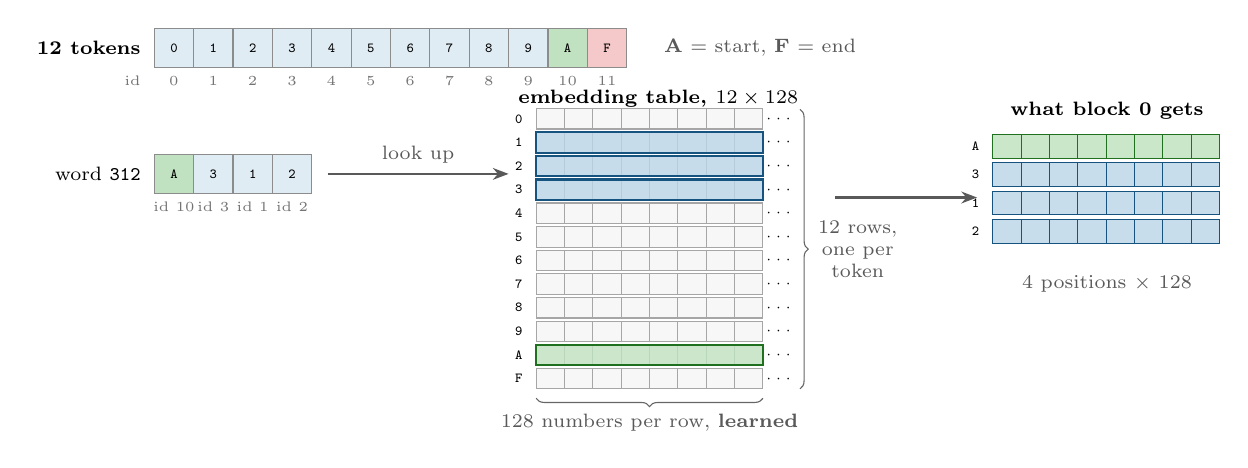
\begin{tikzpicture}
  % the alphabet
  \node[font=\scriptsize\bfseries, anchor=east] at (-0.3,0) {12 tokens};
  \cellrow{0}{0}{0.5}{0/cd,1/cd,2/cd,3/cd,4/cd,5/cd,6/cd,7/cd,8/cd,9/cd,A/cs,F/ce}
  \foreach \i in {0,...,11} {\node[font=\tiny, text=black!55] at (\i*0.5,-0.42) {\i};}
  \node[font=\tiny, text=black!55, anchor=east] at (-0.3,-0.42) {id};
  \node[note, anchor=west] at (6.1,0) {\textbf{A} = start, \textbf{F} = end};

  % a word becomes ids
  \node[font=\scriptsize, anchor=east] at (-0.3,-1.6) {word \texttt{312}};
  \cellrow{0}{-1.6}{0.5}{A/cs,3/cd,1/cd,2/cd}
  \foreach \v [count=\i from 0] in {10,3,1,2} {\node[font=\tiny, text=black!55] at (\i*0.5,-2.02) {id \v};}

  % the embedding table
  \begin{scope}[shift={(4.6,-0.9)}]
    \node[font=\scriptsize\bfseries] at (1.55,0.25) {embedding table, $12\times128$};
    \foreach \r [count=\k from 0] in {0,1,2,3,4,5,6,7,8,9,A,F} {
      \pgfmathsetmacro{\yy}{-\k*0.3}
      \node[font=\tiny\ttfamily, anchor=east] at (-0.05,\yy) {\r};
      \foreach \c in {0,...,7} {\draw[black!35, fill=black!3] (\c*0.36,\yy-0.13) rectangle ++(0.36,0.26);}
      \node[font=\tiny] at (3.1,\yy) {$\cdots$};
    }
    % highlight rows A,3,1,2
    \foreach \k/\col in {10/okgreen, 3/validblue, 1/validblue, 2/validblue} {
      \fill[\col!30, opacity=0.8] (0,-\k*0.3-0.13) rectangle ++(2.88,0.26);
      \draw[\col!70!black, thick] (0,-\k*0.3-0.13) rectangle ++(2.88,0.26);
    }
    \draw[br] (3.35,0.12) -- (3.35,-3.43) node[midway, right=3pt, note] {12 rows,\\one per\\token};
    \draw[br] (2.88,-3.55) -- (0,-3.55) node[midway, below=2pt, note] {128 numbers per row, \textbf{learned}};
  \end{scope}
  \draw[arr] (1.95,-1.6) -- node[above, note] {look up} (4.25,-1.6);

  % output vectors
  \begin{scope}[shift={(10.4,-1.25)}]
    \node[font=\scriptsize\bfseries] at (1.45,0.45) {what block 0 gets};
    \foreach \r/\col [count=\k from 0] in {A/okgreen,3/validblue,1/validblue,2/validblue} {
      \node[font=\tiny\ttfamily, anchor=east] at (-0.05,-\k*0.36) {\r};
      \foreach \c in {0,...,7} {\draw[\col!70!black, fill=\col!25] (\c*0.36,-\k*0.36-0.15) rectangle ++(0.36,0.3);}
    }
    \node[note] at (1.45,-1.75) {4 positions $\times$ 128};
  \end{scope}
  \draw[arr] (8.4,-1.9) -- (10.2,-1.9);
\end{tikzpicture}

\vspace{1mm}
\begin{itemize}\small
\item The network never sees that \texttt{3} means three. To it, \texttt{3} is whatever vector sits in row 3; training moves the rows.
\item The code multiplies a one-hot matrix by the table (same rows, same FP32 values) instead of calling \code{nn.Embedding}: the lookup kernel hangs NVBit.
\end{itemize}
\end{frame}

%-----------------------------------------------------------------------------
\begin{frame}{Where the batch size 100 comes from: one row per training word}
\centering
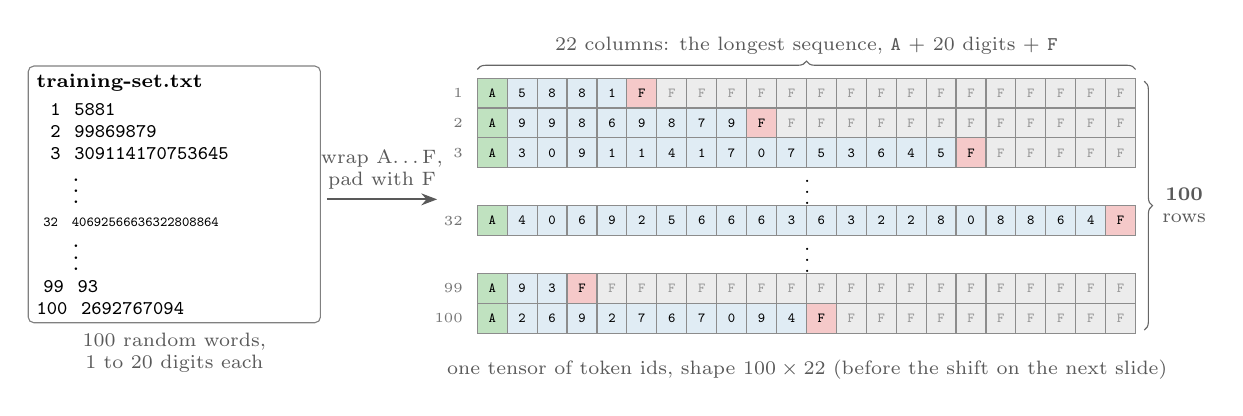
\begin{tikzpicture}
  % the file
  \node[card, anchor=north west, font=\scriptsize\ttfamily, text width=3.5cm] (file) at (-0.6,0.35) {%
    \textrm{\textbf{training-set.txt}}\\[2pt]
    \ \ 1\ \ 5881\\
    \ \ 2\ \ 99869879\\
    \ \ 3\ \ 309114170753645\\
    \ \ \ \ \ $\vdots$\\
    {\tiny\ 32\ \ 40692566636322808864}\\
    \ \ \ \ \ $\vdots$\\
    \ 99\ \ 93\\
    100\ \ 2692767094};
  \node[note, anchor=north] at (file.south) {100 random words,\\1 to 20 digits each};

  \draw[arr] (3.2,-1.35) -- node[above, note] {wrap A\dots F,\\pad with F} (4.6,-1.35);

  % the batch
  \def\w{0.38}
  \begin{scope}[shift={(5.3,0)}]
    \cellrow{0}{0}{\w}{A/cs,5/cd,8/cd,8/cd,1/cd,F/ce,F/cp,F/cp,F/cp,F/cp,F/cp,F/cp,F/cp,F/cp,F/cp,F/cp,F/cp,F/cp,F/cp,F/cp,F/cp,F/cp}
    \cellrow{0}{-\w}{\w}{A/cs,9/cd,9/cd,8/cd,6/cd,9/cd,8/cd,7/cd,9/cd,F/ce,F/cp,F/cp,F/cp,F/cp,F/cp,F/cp,F/cp,F/cp,F/cp,F/cp,F/cp,F/cp}
    \cellrow{0}{-2*\w}{\w}{A/cs,3/cd,0/cd,9/cd,1/cd,1/cd,4/cd,1/cd,7/cd,0/cd,7/cd,5/cd,3/cd,6/cd,4/cd,5/cd,F/ce,F/cp,F/cp,F/cp,F/cp,F/cp}
    \node[font=\scriptsize] at (4.0,-3*\w-0.02) {$\vdots$};
    \cellrow{0}{-4*\w-0.1}{\w}{A/cs,4/cd,0/cd,6/cd,9/cd,2/cd,5/cd,6/cd,6/cd,6/cd,3/cd,6/cd,3/cd,2/cd,2/cd,8/cd,0/cd,8/cd,8/cd,6/cd,4/cd,F/ce}
    \node[font=\scriptsize] at (4.0,-5*\w-0.12) {$\vdots$};
    \cellrow{0}{-6*\w-0.2}{\w}{A/cs,9/cd,3/cd,F/ce,F/cp,F/cp,F/cp,F/cp,F/cp,F/cp,F/cp,F/cp,F/cp,F/cp,F/cp,F/cp,F/cp,F/cp,F/cp,F/cp,F/cp,F/cp}
    \cellrow{0}{-7*\w-0.2}{\w}{A/cs,2/cd,6/cd,9/cd,2/cd,7/cd,6/cd,7/cd,0/cd,9/cd,4/cd,F/ce,F/cp,F/cp,F/cp,F/cp,F/cp,F/cp,F/cp,F/cp,F/cp,F/cp}
    \foreach \n/\y in {1/0, 2/-\w, 3/-2*\w, 32/-4*\w-0.1, 99/-6*\w-0.2, 100/-7*\w-0.2}
      {\node[font=\tiny, text=black!55, anchor=east] at (-0.25,\y) {\n};}
    \draw[br] (21*\w+0.3,0.15) -- (21*\w+0.3,-7*\w-0.35) node[midway, right=3pt, note] {\textbf{100}\\rows};
    \draw[br] (-0.19,0.3) -- (21*\w+0.19,0.3) node[midway, above=2pt, note] {22 columns: the longest sequence, \texttt{A} + 20 digits + \texttt{F}};
    \node[note, anchor=north] at (4.0,-7*\w-0.6) {one tensor of token ids, shape $100\times22$ (before the shift on the next slide)};
  \end{scope}
\end{tikzpicture}

\vspace{2mm}
\small
\legendcell{cs}{A} start \quad \legendcell{cd}{5} digit \quad \legendcell{ce}{F} end \quad \legendcell{cp}{F} padding\\[2mm]
\raggedright
There is no batch-size setting: \code{train.py} stacks \emph{every} word of the training set into one batch and
takes all 1500 optimizer steps on that same batch (no shuffling, no sampling).
\end{frame}

%-----------------------------------------------------------------------------
\begin{frame}{Where 21 comes from: each position predicts the next token}
\centering
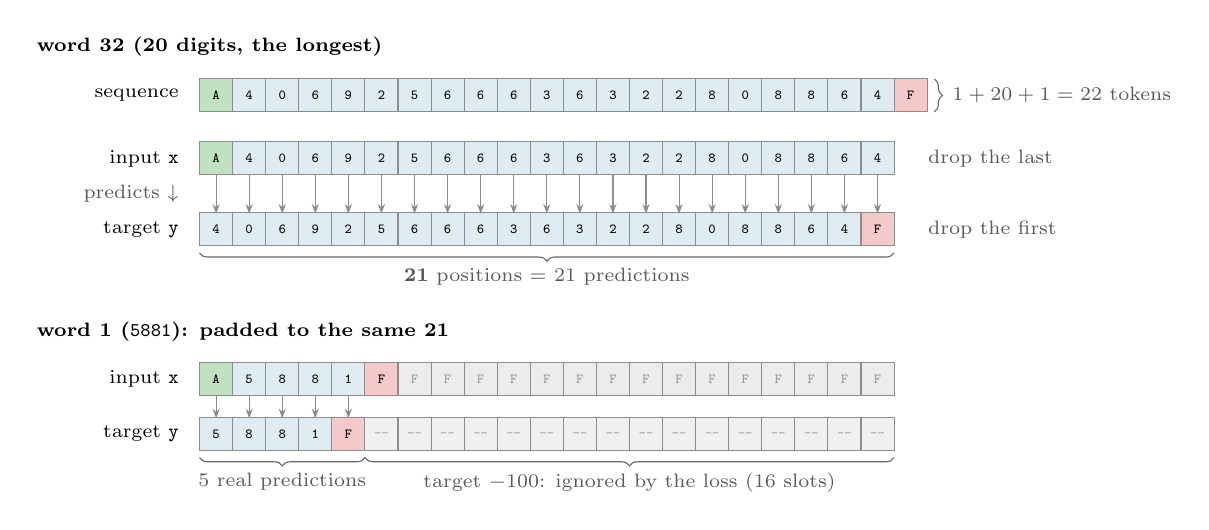
\begin{tikzpicture}
  \def\w{0.42}
  % longest word
  \node[font=\scriptsize\bfseries, anchor=west] at (-2.4,0.62) {word 32 (20 digits, the longest)};
  \node[font=\scriptsize, anchor=east] at (-0.35,0) {sequence};
  \cellrow{0}{0}{\w}{A/cs,4/cd,0/cd,6/cd,9/cd,2/cd,5/cd,6/cd,6/cd,6/cd,3/cd,6/cd,3/cd,2/cd,2/cd,8/cd,0/cd,8/cd,8/cd,6/cd,4/cd,F/ce}
  \draw[br] (21*\w+0.3,0.21) -- (21*\w+0.3,-0.21) node[midway, right=3pt, note, align=left] {$1+20+1 = 22$ tokens};

  \node[font=\scriptsize, anchor=east] at (-0.35,-0.8) {input \texttt{x}};
  \cellrow{0}{-0.8}{\w}{A/cs,4/cd,0/cd,6/cd,9/cd,2/cd,5/cd,6/cd,6/cd,6/cd,3/cd,6/cd,3/cd,2/cd,2/cd,8/cd,0/cd,8/cd,8/cd,6/cd,4/cd}
  \node[note, anchor=west] at (21*\w+0.1,-0.8) {drop the last};
  \node[font=\scriptsize, anchor=east] at (-0.35,-1.7) {target \texttt{y}};
  \cellrow{0}{-1.7}{\w}{4/cd,0/cd,6/cd,9/cd,2/cd,5/cd,6/cd,6/cd,6/cd,3/cd,6/cd,3/cd,2/cd,2/cd,8/cd,0/cd,8/cd,8/cd,6/cd,4/cd,F/ce}
  \node[note, anchor=west] at (21*\w+0.1,-1.7) {drop the first};
  \foreach \i in {0,...,20} {\draw[-{Stealth[length=1.2mm]}, black!45] (\i*\w,-1.0) -- (\i*\w,-1.5);}
  \node[note, anchor=east] at (-0.35,-1.25) {predicts $\downarrow$};
  \draw[br] (20*\w+0.21,-2.0) -- (-0.21,-2.0) node[midway, below=2pt, note] {\textbf{21} positions = 21 predictions};

  % short word
  \node[font=\scriptsize\bfseries, anchor=west] at (-2.4,-3.0) {word 1 (\texttt{5881}): padded to the same 21};
  \node[font=\scriptsize, anchor=east] at (-0.35,-3.6) {input \texttt{x}};
  \cellrow{0}{-3.6}{\w}{A/cs,5/cd,8/cd,8/cd,1/cd,F/ce,F/cp,F/cp,F/cp,F/cp,F/cp,F/cp,F/cp,F/cp,F/cp,F/cp,F/cp,F/cp,F/cp,F/cp,F/cp}
  \node[font=\scriptsize, anchor=east] at (-0.35,-4.3) {target \texttt{y}};
  \cellrow{0}{-4.3}{\w}{5/cd,8/cd,8/cd,1/cd,F/ce,--/cx,--/cx,--/cx,--/cx,--/cx,--/cx,--/cx,--/cx,--/cx,--/cx,--/cx,--/cx,--/cx,--/cx,--/cx,--/cx}
  \foreach \i in {0,...,4} {\draw[-{Stealth[length=1.2mm]}, black!45] (\i*\w,-3.8) -- (\i*\w,-4.1);}
  \draw[br] (20*\w+0.21,-4.6) -- (5*\w-0.21,-4.6) node[midway, below=2pt, note] {target $-100$: ignored by the loss (16 slots)};
  \draw[br] (4*\w+0.21,-4.6) -- (-0.21,-4.6) node[midway, below=2pt, note] {5 real predictions};
\end{tikzpicture}

\vspace{1mm}
\small So the training batch is $100 \times 21$: 100 words, 21 positions each.
\end{frame}

%-----------------------------------------------------------------------------
\begin{frame}{The batch on its way into attention}
\centering
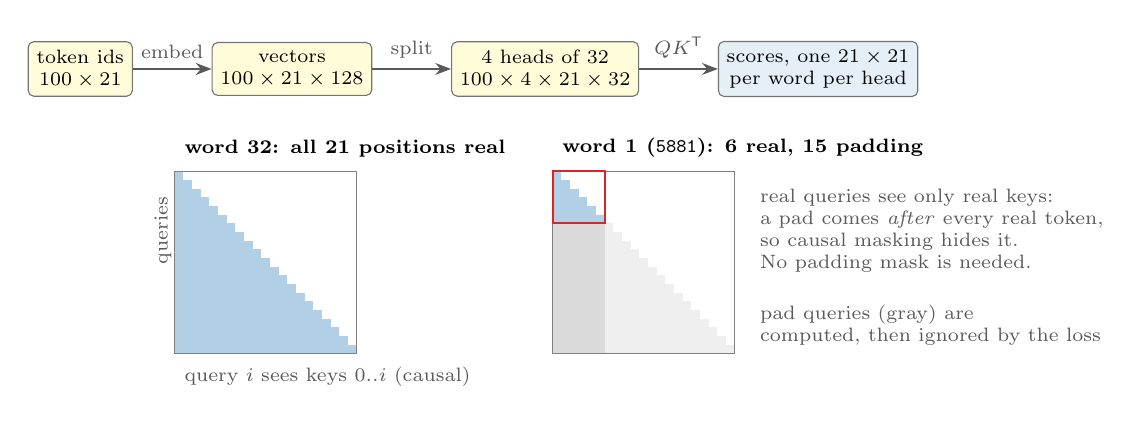
\begin{tikzpicture}
  \node[shp] (ids) at (0,0) {token ids\\$100\times21$};
  \node[shp, right=1.0cm of ids] (emb) {vectors\\$100\times21\times128$};
  \node[shp, right=1.0cm of emb] (heads) {4 heads of 32\\$100\times4\times21\times32$};
  \node[shp, right=1.0cm of heads, fill=validblue!12] (sc) {scores, one $21\times21$\\per word per head};
  \draw[arr] (ids) -- node[above, note] {embed} (emb);
  \draw[arr] (emb) -- node[above, note] {split} (heads);
  \draw[arr] (heads) -- node[above, note] {$QK^{\mathsf T}$} (sc);

  % two score grids
  \def\c{0.11}
  \begin{scope}[shift={(1.2,-1.3)}]
    \node[font=\scriptsize\bfseries, anchor=south west] at (0,0.05) {word 32: all 21 positions real};
    \foreach \r in {0,...,20} { \foreach \k in {0,...,20} {
      \ifnum\k>\r \def\f{white}\else \def\f{validblue!35}\fi
      \fill[\f] (\k*\c,-\r*\c-\c) rectangle ++(\c,\c); } }
    \draw[black!50] (0,0) rectangle (21*\c,-21*\c);
    \node[note, anchor=north west] at (0,-21*\c-0.05) {query $i$ sees keys $0..i$ (causal)};
    \node[note, anchor=east, rotate=90] at (-0.15,-0.2) {queries};
    \node[note, anchor=west] at (0,0.0) {};
  \end{scope}
  \begin{scope}[shift={(6.0,-1.3)}]
    \node[font=\scriptsize\bfseries, anchor=south west] at (0,0.05) {word 1 (\texttt{5881}): 6 real, 15 padding};
    \foreach \r in {0,...,20} { \foreach \k in {0,...,20} {
      \ifnum\k>\r \def\f{white}\else
        \ifnum\r<6 \def\f{validblue!35}\else
          \ifnum\k<6 \def\f{padgray!35}\else \def\f{padgray!15}\fi\fi\fi
      \fill[\f] (\k*\c,-\r*\c-\c) rectangle ++(\c,\c); } }
    \draw[black!50] (0,0) rectangle (21*\c,-21*\c);
    \draw[nanred, thick] (0,0) rectangle (6*\c,-6*\c);
    \node[note, anchor=west, align=left] at (21*\c+0.2,-0.75) {real queries see only real keys:\\a pad comes \emph{after} every real token,\\so causal masking hides it.\\No padding mask is needed.};
    \node[note, anchor=west, align=left] at (21*\c+0.2,-1.95) {pad queries (gray) are\\computed, then ignored by the loss};
  \end{scope}
\end{tikzpicture}

\vspace{2mm}
\begin{columns}[T]
\column{0.5\textwidth}\small
\textbf{Training} (\code{train.py}): $100\times4 = 400$ score grids of $21\times21$ in each of the 4 blocks,
every step, on the same batch for all 1500 steps.
\column{0.46\textwidth}\small
\textbf{Generation} (\code{generate.py}): batch \textbf{1}. Prompt \texttt{A312} is one call ($1\times4\times4\times32$),
then one call per new token, attending over the stored keys: up to 7 positions.
\end{columns}
\end{frame}

\end{document}
